\documentclass[12pt, twoside]{article}
\usepackage[letterpaper, margin=1in, headsep=0.5in]{geometry}
\usepackage[english]{babel}
\usepackage[utf8]{inputenc}
\usepackage{amsmath}
\usepackage{amsfonts}
\usepackage{amssymb}
\usepackage{tikz}
%\usetikzlibrary{quotes, angles}

\usepackage{graphicx}
\usepackage{enumitem}
\usepackage{multicol}

\usepackage{fancyhdr}
\pagestyle{fancy}
\fancyhf{}
\renewcommand{\headrulewidth}{0pt} % disable the underline of the header

\fancyhead[RE]{\thepage}
\fancyhead[RO]{\thepage \\ Name: \hspace{3cm}}
\fancyhead[L]{BECA / Dr. Huson / 10th Grade Geometry\\* Unit 8 Transformations\\19 March 2019}

\begin{document}
\subsubsection*{8-12 Regents Geometric Situations}
  \begin{enumerate}

  \item After a dilation with center $(0,0)$, the image of $\overline{MN}$ is $\overline{M'N'}$. If $MN=4.5$ and $M'N'=18$, find the scale factor of this dilation.

  \item In the diagram below, $\triangle ABC$ with sides of 13, 15, and 16, is mapped onto $\triangle DEF$ after a clockwise rotation of $90^\circ$ about point $P$.
    \begin{center}
      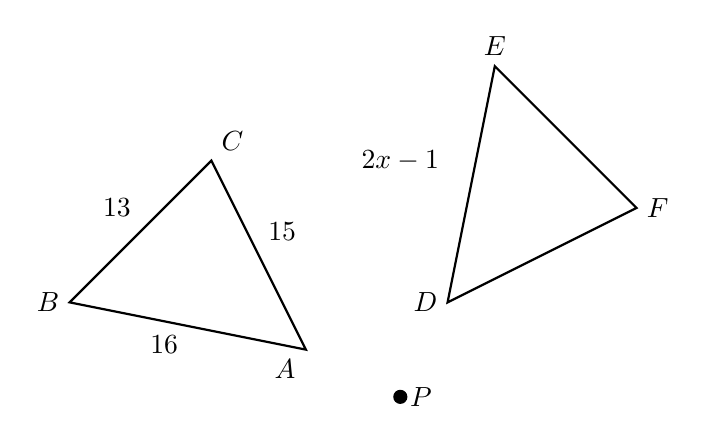
\begin{tikzpicture}[scale=.6]
      %\draw [thick, <->] (-7.4,0) -- (10.4,0) node [right] {$x$};
      %draw [thick, <->] (0,-5.4)--(0,10.4) node [above] {$y$};
      \fill (0,0) circle[radius=0.15] node[right]{$P$};
        \draw [thick]
        (-2,1) node[below left] {$A$}--
        (-7,2) node[left] {$B$}--
        (-4,5) node[above right] {$C$}--cycle;
          \node at (-5,1.5)[below]{16};
          \node at (-6,4){13};
          \node at (-2.5,3.5){15};
          \node at (0,5){$2x-1$};
        \draw [thick]
        (1,2) node[left] {$D$}--
        (2,7) node[above] {$E$}--
        (5,4) node[right] {$F$}--cycle;
      \end{tikzpicture}
    \end{center}

    If $DE=2x-1$, what is the value of $x$?

  \item On the set of axes below, $\triangle ABC$ has vertices at $A(-2,0)$, $B(2,4)$, $C(4,2)$, and $\triangle DEF$ has vertices at $D(4,0)$, $E(-4,8)$, $F(-8,-4)$.
    [10 by 10 graph, labeled vertices]

    Mark each statement True or False
      \begin{enumerate}
        \item A dilation with a scale factor of 2 centered at point $A$ maps $\triangle ABC \rightarrow \triangle DEF$ \hfill True \quad False
        \item A dilation with a scale factor of $\frac{1}{2}$ centered at point $A$ maps $\triangle ABC \rightarrow \triangle DEF$ \hfill True \quad False
        \item A dilation with a scale factor of 2 centered at the origin, followed by a rotation of $180^\circ$ about the origin maps $\triangle ABC \rightarrow \triangle DEF$ \hfill True \quad False
      \end{enumerate}

    \item The figure shows a rhombus with noncongruent diagonals.

    True or False? The given transformation carries the rhombus onto itself.
      \begin{enumerate}
        \item A reflection over the shorter diagonal \hfill True \quad False
        \item A reflection over the longer diagonal \hfill True \quad False
        \item A clockwise rotation of $90^\circ$ about the intersection of the diagonals \hfill True \quad False
        \item A clockwise rotation of $180^\circ$ about the intersection of the diagonals \hfill True \quad False
      \end{enumerate}

    \item In right triangle $ABC$ shown below, point $D$ is on $\overline{AB}$ and point $E$ is on $\overline{BC}$ such that $\overline{AC} \parallel \overline{DE}$
    [right triangles]
    If $AB=15$, $BC=12$, and $EC=7$, what is the length of $\overline{BD}$?


  \end{enumerate}

  \end{document}
